\chapter{State of the Art} \label{chap:State of the Art}
Chapter HEader

\section{Implementation of Reactive Systems}

\subsection{Observer Design Pattern}


\subsection{Aspect-Oriented Programming} \label{subsec:AOP}

\subsection{Callbacks}

\subsection{Promises}

\subsection{Iterator Vs Observer Pattern}


\section{Reactive Programming}

\subsection{Reactive Programming with JavaScript}


\subsection{ReactiveX and RxJS}

\subsection{Important Concepts of RxJS}

\begin{figure}[!h]
	\centering
	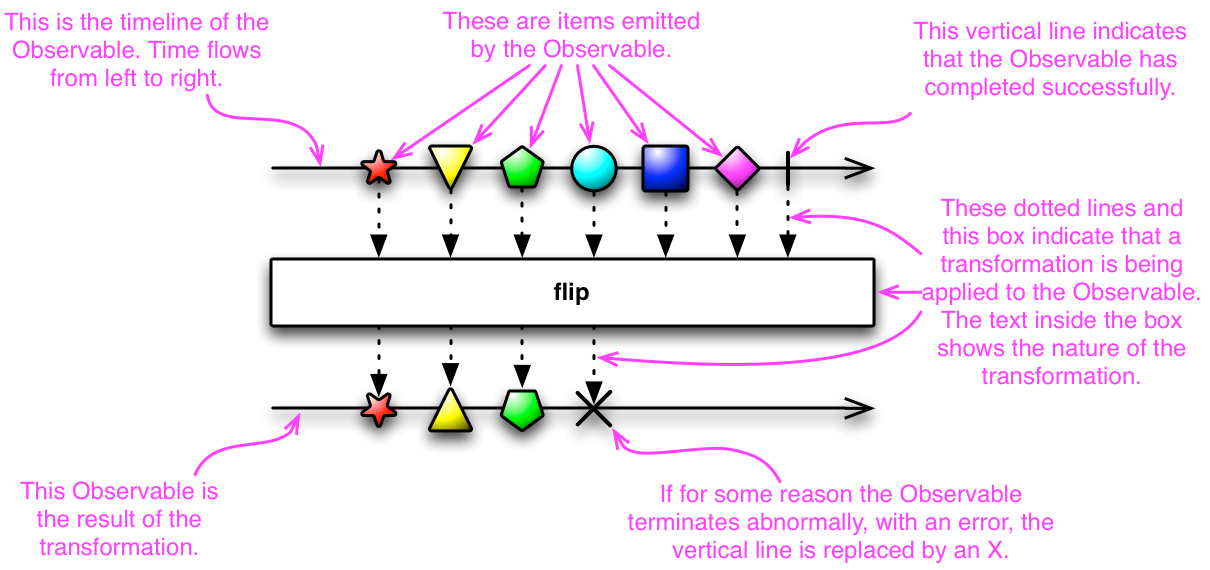
\includegraphics[scale=0.5,trim=0 0 0 0]{gfx/rxjs-reactive-pattern2.png}
	\caption{Reactive pattern \protect\cite{ReactiveXobservable}}
	\label{fig:rxjs-reactive-pattern}
\end{figure}

\textbf{Observable and Observer}\\
Placeholder

\textbf{Operators}
\label{subsec:Operators}\\

\textbf{RxJS Code Structure}\\
Placeholder
\begin{lstlisting}[language=JavaScript, caption=RxJS Simple Example, label={lst:RxJS_Simple_Example}]
// 1. Srouce Observable Creation
var sourceObservable = Rx.Observable.interval(1000);
// 2. Transformation by applying different operators
var transformedObservable = sourceObservable.map(function(x) {
		return x * 10;
	})
	.filter(function(x) {
		return x !== 20
	})
	.take(5);
// 3. Subscribe to desired Observable 
var subscription = transformedObservable.subscribe(
	function(x) {
		console.log('Next: ' + x);
	},
	function(err) {
		console.log('Error: ' + err);
	},
	function() {
		console.log('Completed');
	});
// OUTPUT
Next: 0
Next: 10
Next: 30
Next: 40
Next: 50
Completed
\end{lstlisting}

\subsection{Bacon.js}

\textbf{EventStream and Property}\\
Placeholder

\section{Debugging and Tools Support}

\subsection{Debugging JavaScript}

\section{Related Work}




